\documentclass[12pt,a4paper]{article}
\usepackage[utf8]{inputenc}
\usepackage{dsfont} 
\usepackage[polish]{babel}
\usepackage{amsmath}
\usepackage{graphicx}
\usepackage[top=1in, bottom=1.5in, left=1.25in, right=1.25in]{geometry}

\usepackage{subfig}
\usepackage{multirow}
\usepackage{multicol}
\graphicspath{{images/}}
\usepackage{xcolor,colortbl}
\usepackage{float}

\newcommand \comment[1]{\textbf{\textcolor{red}{#1}}}

%\usepackage{float}
\usepackage{fancyhdr} % Required for custom headers
\usepackage{lastpage} % Required to determine the last page for the footer
\usepackage{extramarks} % Required for headers and footers
\usepackage{indentfirst}
\usepackage{placeins}
\usepackage{scalefnt}
\usepackage{xcolor,listings}
\usepackage{textcomp}
\usepackage{color}
\usepackage{verbatim}
\usepackage{framed}
\usepackage[T1]{fontenc}

\definecolor{codegreen}{rgb}{0,0.6,0}
\definecolor{codegray}{rgb}{0.5,0.5,0.5}
\definecolor{codepurple}{HTML}{C42043}
\definecolor{backcolour}{HTML}{F2F2F2}
\definecolor{bookColor}{cmyk}{0,0,0,0.90}  
\color{bookColor}

\lstset{upquote=true}

\lstdefinestyle{mystyle}{
	backgroundcolor=\color{backcolour},   
	commentstyle=\color{codegreen},
	keywordstyle=\color{codepurple},
	numberstyle=\numberstyle,
	stringstyle=\color{codepurple},
	basicstyle=\footnotesize\ttfamily,
	breakatwhitespace=false,
	breaklines=true,
	captionpos=b,
	keepspaces=true,
	numbers=left,
	numbersep=10pt,
	showspaces=false,
	showstringspaces=false,
	showtabs=false,
}
\lstset{style=mystyle}

\newcommand\numberstyle[1]{%
	\footnotesize
	\color{codegray}%
	\ttfamily
	\ifnum#1<10 0\fi#1 |%
}

\definecolor{shadecolor}{HTML}{F2F2F2}

\newenvironment{sqltable}%
{\snugshade\verbatim}%
{\endverbatim\endsnugshade}

% Margins
\addtolength{\footskip}{0cm}
\addtolength{\textwidth}{1.4cm}
\addtolength{\oddsidemargin}{-.7cm}

\addtolength{\textheight}{1.6cm}
%\addtolength{\topmargin}{-2cm}

% paragrafo
\addtolength{\parskip}{.2cm}

% Set up the header and footer
\pagestyle{fancy}
\rhead{\hmwkAuthorName} % Top left header
\lhead{\hmwkClass: \hmwkTitle} % Top center header
\rhead{\firstxmark} % Top right header
\lfoot{Maria Koren, Mateusz Domino} % Bottom left footer
\cfoot{} % Bottom center footer
\rfoot{} % Bottom right footer
\renewcommand{\headrulewidth}{1pt}
\renewcommand{\footrulewidth}{1pt}

    
\newcommand{\hmwkTitle}{Niezdecydowany więdrowiec} % Tytuł projektu
\newcommand{\hmwkDueDate}{\today} % Data 
\newcommand{\hmwkClass}{Algorytmy Numeryczne} % Nazwa przedmiotu
\newcommand{\hmwkAuthorName}{Maria Koren, Mateusz Domino} % Imię i nazwisko

% trabalho 
\begin{document}
% capa
\begin{titlepage}
    \vfill
	\begin{center}
	\hspace*{-1cm}
	\vspace*{0.5cm}
    \includegraphics[scale=0.55]{images/loga.png}\\
	\textbf{Uniwersytet Gdański \\ [0.05cm]Wydział Matematyki, Fizyki i Informatyki \\ [0.05cm] Instytut Informatyki}

	\vspace{0.6cm}
	\vspace{4cm}
	{\huge \textbf{\hmwkTitle}}\vspace{8mm}
	
	{\large \textbf{\hmwkAuthorName}}\\[3cm]
	

	  \vfill
	%\vspace{2cm}
	
	\textbf{Gdańsk}
	
	\textbf{\hmwkDueDate}
	\end{center}
	
\end{titlepage}

\newpage
\setcounter{secnumdepth}{5}
\tableofcontents
\newpage

\section{Opis zadania}
W zadaniu rozważono spacerującego wędrowca. Park, w którym spaceruje wędrowiec, składa się z alejek oraz  skrzyżowań tych alejek. W dalszym zadaniu przyjęto że to jest graf, w którym każdy krok jest osobnym wierszchołkiem. Przykładowy graf jest na rysunku \ref{fig:przykladowygraf}. W tym parku alejki pomiędzy skrzyżowaniami 1 a 2, 2 a 3, 3 a 4, 4 a 1 mają po 4 kroki, natomiast alejka łącząca skrzyżowania 1 a 3 ma 6 kroków.

\begin{figure}[h]
  \centering
  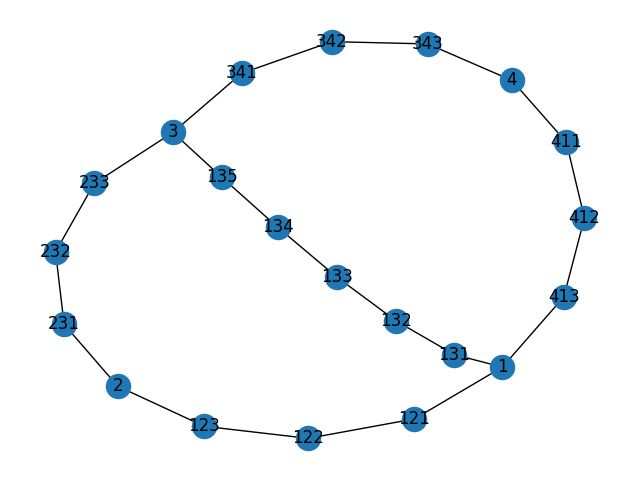
\includegraphics[width=0.5\textwidth]{images/przykladowygraf.png}
  \caption{Przykładowy graf}
  \label{fig:przykladowygraf}
\end{figure}

Niezdecydowany wędrowiec spacerując parkiem spaceruje wędług tych kroków, wybierając z jednakowym prawdopodobieństwem każdy z możliwych kroków (na grafie to oznacza każdy z sąsiędnich wierszchołków). W jednym z wierszchołków jest wyjście, w innym jest OSK (odkryta studzienka kanalizacyjna), na której kończy się spacer. Przykładowo można założyć, że OSK jest w punkcie 5, wyjście w punkcie 2, natomiast wędrowiec startuje z punkta 4. 

Trzeba obliczyć prawdopodobieństwo bezpiecznego powrotu do domu, inaczej mówiąc prawdopodobieństwo że wędrowiec dojdzie do punkta z wyjściem.

\newpage
\section{Symulacja wędrowki}
Została zaimplementowana symulacja wędrowki. W tym celu użyto metody Monte Carlo. W napisanej symulacji wędrowca ustawiamy w punkt startowy. Zatem spośród sąsiadujących z aktualnym wierszchołkiem losowano kolejny wierszchołek do którego wędrowca pójdzie dalej i zmieniano aktualny wierszchołek na ten następny. Sprawdzano czy to jest wyjście czy osk, jeżeli nie, idzie wędrowca dalej, jeżeli wyjście  --- zwiększano licznik podróż zakończonych sukcesem i koniec symulacji, jeżeli osk --- zwiększano licznik podróż zakończonych porażką i koniec symulacji.

Zatem obliczono procent ze wszystkuch podróż startujących z tego samego miejsca zakończonych sukcesem. Jest to prawdopodobieństwo bezpiecznego powrotu do doma.

\newpage
\section{Budowanie układu równań}

W celu rozwiązania powyższego promlemu zrobiono macierz oznaczającą układ równań. Dla powyższego przykładu macierz wygląda następująco:

\begin{figure}[h]
  \centering
  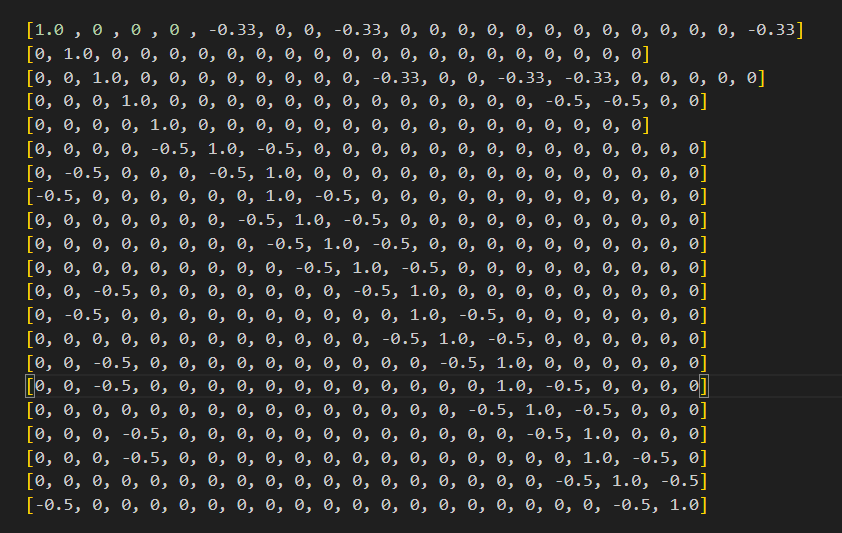
\includegraphics[width=10cm]{images/macierz.png}
  \caption{Macierz}
  \label{fig:macierz}
\end{figure}

Kolumna wyrazów wolnych dla układu równań wygląda tak, że są to same 0, oprócz miejsca w którym jest wyjście.

Rozwiązując taki układ równań otrzymano rozwiązanie. Rozwiązywanie takiego układu równań daje listę prawdopodobieństw, że wędrowiec będzie mógł bezpiecznie wrócić z parku jeżeli startuje w każdym z punktów.

Dla powyższego przykładu lista rozwiązań wygląda w taki sposób: 

[0.11864406779661008, 1.0, 0.5254237288135589, 0.32203389830508455, 0.0, \\
0.3333333333333333, 0.6666666666666666, 0.18644067796610156, 0.25423728813559304, \\
0.3220338983050845, 0.38983050847457595, 0.4576271186440674, 0.8813559322033897, \\
0.7627118644067794, 0.6440677966101691, 0.4745762711864403, 0.4237288135593218, \\
0.3728813559322032, 0.271186440677966, 0.22033898305084737, 0.1694915254237287]

W podanym przykładzie wędrowiec startował z punktu 4, więc prawdopodobieństwo że bezbiecznie wróci do domu wynosi \textbf{0.32203389830508455}.


W celu tworzenia takiej macierzy był napisany program w języku python (\textit{podstawowa.py}). Ten program najpierw wczytuje dane o skrzyżowaniach i ilości kroków między nimi, na tej podstawie buduje graf. Zatem tworzy tak zwaną macierz sąsiędstw. Po tym buduje układ równań, opisujący możliwe przejścia pomiędzy wierszchołkami. Dalej program wczytywa informacje odnośnie osk oraz wyjścia i następnie korektuje tą macierz.


\newpage
\section{Algorytmy rozwiązywania układów równań}

Zostały napisane 3 algorytmy, rozwiązujące układy równań.

\subsection{Algorytm eliminacji Gaussa bez wyboru elementa podstawowego}

Algorytm eliminacji Gaussa najpierw przekształca macierz za pomocą odpowiednich operacji elementarnych takich jak dodawanie, odejmowanie i mnożenie wierszy, aby sprowadzić macierz do postaci trójkątnej górnej. A potem za pomocą postępowania odwrotnego znajduje rozwiązania dla zmiennych.

\subsection{Algorytm eliminacji Gaussa z częściowym wyborem  elementu podstawowego}

Algorytm Gaussa z częściowym wyborem elementu podstawowego jest ulepszeniem podstawowego algorytmu eliminacji Gaussa używanego do rozwiązywania układów równań liniowych.  Algorytm Gaussa z częściowym wyborem elementu podstawowego polega na wyborze największego elementu w kolumnie jako elementu podstawowego. Jest to wykonane przed dokonaniem eliminacji Gaussa. Ten proces zapobiega zerowaniu się głównych elementów na przekątnej, co z kolei pozwala na uniknięcie konieczności zmiany kolejności równań.

\subsection{Metoda iteracyjna Gaussa-Seidela}

Jest to technika iteracyjna, która polega na rozwiązaniu układu równań poprzez iteracyjne poprawianie wartości niewiadomych w każdej iteracji. Najpierw jest wybierane początkowe przybliżenie. Zatem iterazyjnie poprawiane to przybliżenie. Koniec iteracji następuje, gdy przybliżenie osiąga pewny poziom przybliżenia, np $10^{-6}$.



\newpage
\section{Hipotezy}
\subsection{Algorytm A2 zwykle daje dokładniejsze wyniki niż A1. Róźnica w dokładności rośnie wraz z rozmiarem macierzy i liczbą niezerowych współczynników}

Pierwszym krokiem weryfikowania hipotezy było użycie macierzy różnych rozmiarów wygenerowanych losowo. Oraz wygenerowanego losowo wektoru wyrazów wolnych. Następnie rozwiązywanie tego układu na 3 sposoby. Wygenerowane lowsowo macierzy nie zawierają zer.
\begin{enumerate}
    \item Za pomocą funkcji wbudowanej
    \item Algorytmem A1
    \item Algorytmem A2
\end{enumerate}
Uważamy że funkcja wbudowana daje idealny wynik. Następnie obliczono różnicę pomiędzy wynikami algorytmu pierwszego a idealnym rozwiązaniem oraz różnicę pomiędzy wynikami algorytmu drugiego a idealnym rozwiązaniem. W celu porównania różnic wyliczono je średnie. 
\begin{table}[h]
\centering
\begin{tabular}{|c|c|c|}
\hline
Rozmiar macierzy & Średnia różnic z algorytmem A1 & Średnia różnic z algorytmem A2  \\
\hline
$100$ & $-2.3918367286768215e-16$ & $-0.0007085089228655519$\\
$200$ & $-5.573666528313482e-17$ & $-0.004144213188631512$\\
$300$ & $-3.8857805861880476e-17$ & $-0.009639807645442993$ \\
$400$ & $4.374972606413507e-17$ & $-0.0012755792202489334 $ \\
$500$ & $-3.2862601528904635e-18$ & $0.011106944930319988$ \\
\hline
\end{tabular}
\caption{Porównanie różnic algorytmu A1 a A2 dla macierzach}
\label{tab:roznicy1}
\end{table}
Z tabeli \ref{tab:roznicy1} wynika, że dla macierzy rozważonych wyżej bez współczynników zerowych najlepsze przybliżenie rozwiązania daje algorytm A1.

Kolejnym krokiem wzięto macierz rzadką, opisującą wędrówkę. Wzięto 4 przyłady grafów. W tym przypadku za idealne rozwiązanie przyjęto wyniki z symulacji Monte Carlo. Wyniki średnich, w zależności od ilości wierszchołków, przedstawiono w tabeli:

\begin{table}[h]
\centering
\begin{tabular}{|c|c|c|}
\hline
Ilość wierszchołków & Średnia różnic z algorytmem A1 & Średnia różnic z algorytmem A2  \\
\hline
$26$ &  $-0.005589991928975173$ & $-0.005589991928975175$\\
$55$ & $0.0006004842615010156$ & $ 0.000600484261501017$\\
$184$ & $-0.001254548059016288$ & $-0.001254548059016297$ \\
$274$ & $-0.0007977564729658342$ & $-0.0007977564729659226$ \\
\hline
\end{tabular}
\caption{Porównanie różnic algorytmu A1 a A2 dla macierzy rzadkich}
\label{tab:roznicy2}
\end{table}

Im większa liczba wierszchołków w grafie tym wieksza jest liczba współczynników zerowych. Więc można zaobserwować że dokładność algorytmu A2 nie zmienia się wraz ze zwiększeniem liczby zerowych współczynników.

Hipoteza 1 o tym, że dokładność algorytmu A2 rośnie wraz ze zwiększeniem rozmiaru macierzy oraz liczbą niezerowych współczynników odrzucona. Przy wzroście niezerowych współczynników oraz rozmiary macierzy algorytm A1 daje dokładniejsze wyniki.

\subsection{Algorytm A3 działa dla postawionego zadania (jeśli nie działa,tzn. proces nie zawsze jest zbieżny do rozwiązania)}

W celu przeprowadzenia testu tej hipotezy, porównano wyniki funkcji wbudowanej z wynikami algorytmu A3 (Gauss'a Siedl'a) ponownie przyjmując, iż funkcja wbudowana zwraca idealne wyniki.

\begin{enumerate}
    \item średniej bezwzględnej różnicy wyników
    \item średniej bezwzględnej różnicy wyników wyrażonej w procentach
    \item maksymalnej bewzględnej różnicy wyników
\end{enumerate}

Przeprowadzono badania na różnych przykładach, stosując algorytm zadania o niezdecydowanym wędrowcu. W każdym modelu studzienka OSK jest na 1, wyjście na 2 a start na 4 skrzyżowaniu. Rozpatrzone przykłady: 

\begin{enumerate}
\item \textbf{Przykład 1:}

\[
\begin{bmatrix}
1 & 2 & 4 \\
2 & 3 & 4 \\
3 & 4 & 4 \\
4 & 1 & 4 \\
1 & 3 & 6 \\
\end{bmatrix}
\]

\textbf{Średnia różnica:} $2.636954938023604e-05$ \\
\textbf{Średnia różnica procentowo:} $0.011096328814801425\%$ \\
\textbf{Max różnica:} $5.137637543317641e-05$

\item \textbf{Przykład 2:}
\[ 
\begin{bmatrix}
1 & 2 & 10 \\
1 & 3 & 15 \\
2 & 3 & 16 \\
3 & 5 & 2 \\
3 & 4 & 8 \\
\end{bmatrix}
\]


\textbf{Średnia różnica:} $0.0010005175219229517$ \\
\textbf{Średnia różnica procentowo:} $0.2571537875924589\%$ \\
\textbf{Max różnica:} $0.002110963264941923$

\newpage

\item \textbf{Przykład 3:}

\[
\begin{bmatrix}
1 & 2 & 20 \\
2 & 3 & 20 \\
3 & 4 & 100 \\
4 & 1 & 10 \\
1 & 3 & 30 \\
\end{bmatrix}
\]

\textbf{Średnia różnica:} $0.10568317608239768$ \\
\textbf{Średnia różnica procentowo:} $45.55101748345425 \%$ \\
\textbf{Max różnica:} $0.21768406594206097$

\item \textbf{Przykładł 4:}

\[
\begin{bmatrix}
1 & 2 & 20 \\
2 & 3 & 20 \\
3 & 4 & 100 \\
4 & 1 & 100 \\
1 & 3 & 30 \\
\end{bmatrix}
\]

\textbf{Średnia różnica:} $0.17209173515787635$ \\
\textbf{Średnia różnica procentowo:} $67.33257287022289 \%$ \\
\textbf{Max różnica:} $0.3429937608772271$

\item \textbf{Przykład 5:}

\[
\begin{bmatrix}
1 & 2 & 2000 \\
2 & 3 & 2000 \\
3 & 4 & 1000 \\
4 & 1 & 1000 \\
1 & 3 & 3000 \\
\end{bmatrix}
\]

\textbf{Średnia różnica:} $0.36014430674617576$ \\
\textbf{Średnia różnica procentowo:} $99.19763545792624 \%$ \\
\textbf{Max różnica:} $0.9545458029087556$
\end{enumerate}

Możemy zauważyć, że czym większa ilość kroków w alejkach, tym algorytm A3 zwraca coraz bardziej rozbieżne wyniki. Ta zależność wynika z rzadkości macierzy w tych przypadkach, co powoduje, że algorytm Gaussa-Siedla nie działa optymalnie.

Hipoteza H2 o tym, że algorytm A3 zawsze działa dla postawionego zadania, odrzucona. Przykłady gdzie proces jest rozbieżny: przykłady 3, 4, 5.

\newpage

\subsection{Jeśli algorytm A3 jest zbieżny do rozwiązania, to wyniki otrzymujemy istotnie szybciej niż dla A1 i A2}

Aby przetestować tę hipotezę użyto dla danych wejściowych, przykłady dla których proces jest zbieżny. Testowanie polegało na pobraniu czasu sprzed i po wykonywaniu funkcji, po czym obliczono czas wykonania każdego algorytmu.

W każdym modelu ponownie studzienka OSK jest na 1, wyjście na 2 a start na 4 skrzyżowaniu.

\textbf{Przykłady:}

\begin{enumerate}
\item \textbf{Przykład 1:}

\[
\begin{bmatrix}
1 & 2 & 4 \\
2 & 3 & 4 \\
3 & 4 & 4 \\
4 & 1 & 4 \\
1 & 3 & 6 \\
\end{bmatrix}
\]

\textbf{Czas wykonywania A1:} $0.00033164024353027344$ sekundy \\
\textbf{Czas wykonywania A2:} $0.00041675567626953125$ sekundy \\
\textbf{Czas wykonywania A3:} $0.00455927848815918$ sekundy

\item \textbf{Przykład 2:}
\[ 
\begin{bmatrix}
1 & 2 & 3 \\
1 & 3 & 2 \\
2 & 3 & 4 \\
3 & 5 & 2 \\
3 & 4 & 5 \\
\end{bmatrix}
\]

\textbf{Czas wykonywania A1:} $0.00014448165893554688$ sekundy  \\
\textbf{Czas wykonywania A2:} $0.00027751922607421875$ sekundy \\
\textbf{Czas wykonywania A3:} $0.004887104034423828$ sekundy

\item \textbf{Przykład 3:}
\[
\begin{bmatrix}
2 & 4 & 1 \\
3 & 5 & 2 \\
1 & 1 & 2 \\
1 & 1 & 5 \\
2 & 3 & 5 \\
\end{bmatrix}
\]

\textbf{Czas wykonywania A1:} $0.00010418891906738281$ sekundy \\
\textbf{Czas wykonywania A2:} $0.00022745132446289062$ sekundy \\
\textbf{Czas wykonywania A3:} $0.004697561264038086$ sekundy
\end{enumerate}

Na podstawie otrzymanych wyników, możemy zauważyć, iż w każdym rozważanym przypadku algorytm A1 i A2 uzyskuje znacznie lepsze wyniki niż algorytm A3.

Hipoteza H3 o szybkości algorytmu A3 dla zbieżnych wyników w porównaniu do A1 oraz A2, odrzucona.

\newpage

\section{Podsumowanie}
W pracy zostało zaimplementowano 3 algorytmy rozwiązywania układów równań. Zweryfikowano 3 hipotezy odnośnie wydajności tych trzech algorytmów.

Poznano macierzy rzadkie oraz sprawdzono na nich efekty algorytmów.
W powyższym zadaniu macierzy rzadkie są wynikiem opisu prawdopodobieństw bezpiecznego powrotu do domu niezdecydowanego wędrowca.

Również zaimplementowano rozszerzenia R0 oraz R1. Może się zdażyć że w parku jest więcej niż jedno wyjście i OSK. Dodatkowo napisana symulacja metodą Monte Carlo. Rozszerzona wersja wraz z metodą Monte Carlo się znajduje w folderze \textit{rozszerzenie}.

\newpage
\section{Zakres pracy}
\begin{itemize}
    \item Maria Koren: implementacja algorytmu A1, podstawowego zadania, metody Monte Carlo weryfikacja hipotezy H1; implementacja rozszerzenia R0
    \item Mateusz Domino: implementacja algorytmów A2 i A3, weryfikacja hipotez H2 i H3;  implementacja rozszerzenia R1
\end{itemize}

\end{document}

